% !TEX root = ../main.tex
% Chapter 1
\flushleft
\chapter{The Showcase}\label{ch:the_showcase} 

Within this section we show examples of VIGRA's
graph API. We believe, most users will use
VIGRA from Python, and therefore we show examples
within Python.
All these examples are shipped with  VIGRA.


\newpage
\paragraph{Agglomerative Clustering}
This examples show how to use  hierarchical /  agglomerative clustering.
We use slic superpixels \citep{achanta_2012_pami}
to get a oversegmentation, and endcode a RAG from that.
We use the mean gradient magnitude between two segments 
of the RAG
as edge indicator/weight.
Furthermore, we use the L1 distance between node features
as additional edge weight.



\lstinputlisting[language=Python,caption={Agglomerative Clustering}]
{/home/tbeier/src/vigra/vigranumpy/examples/graph_agglomerative_clustering.py}
\begin{figure}
\centering
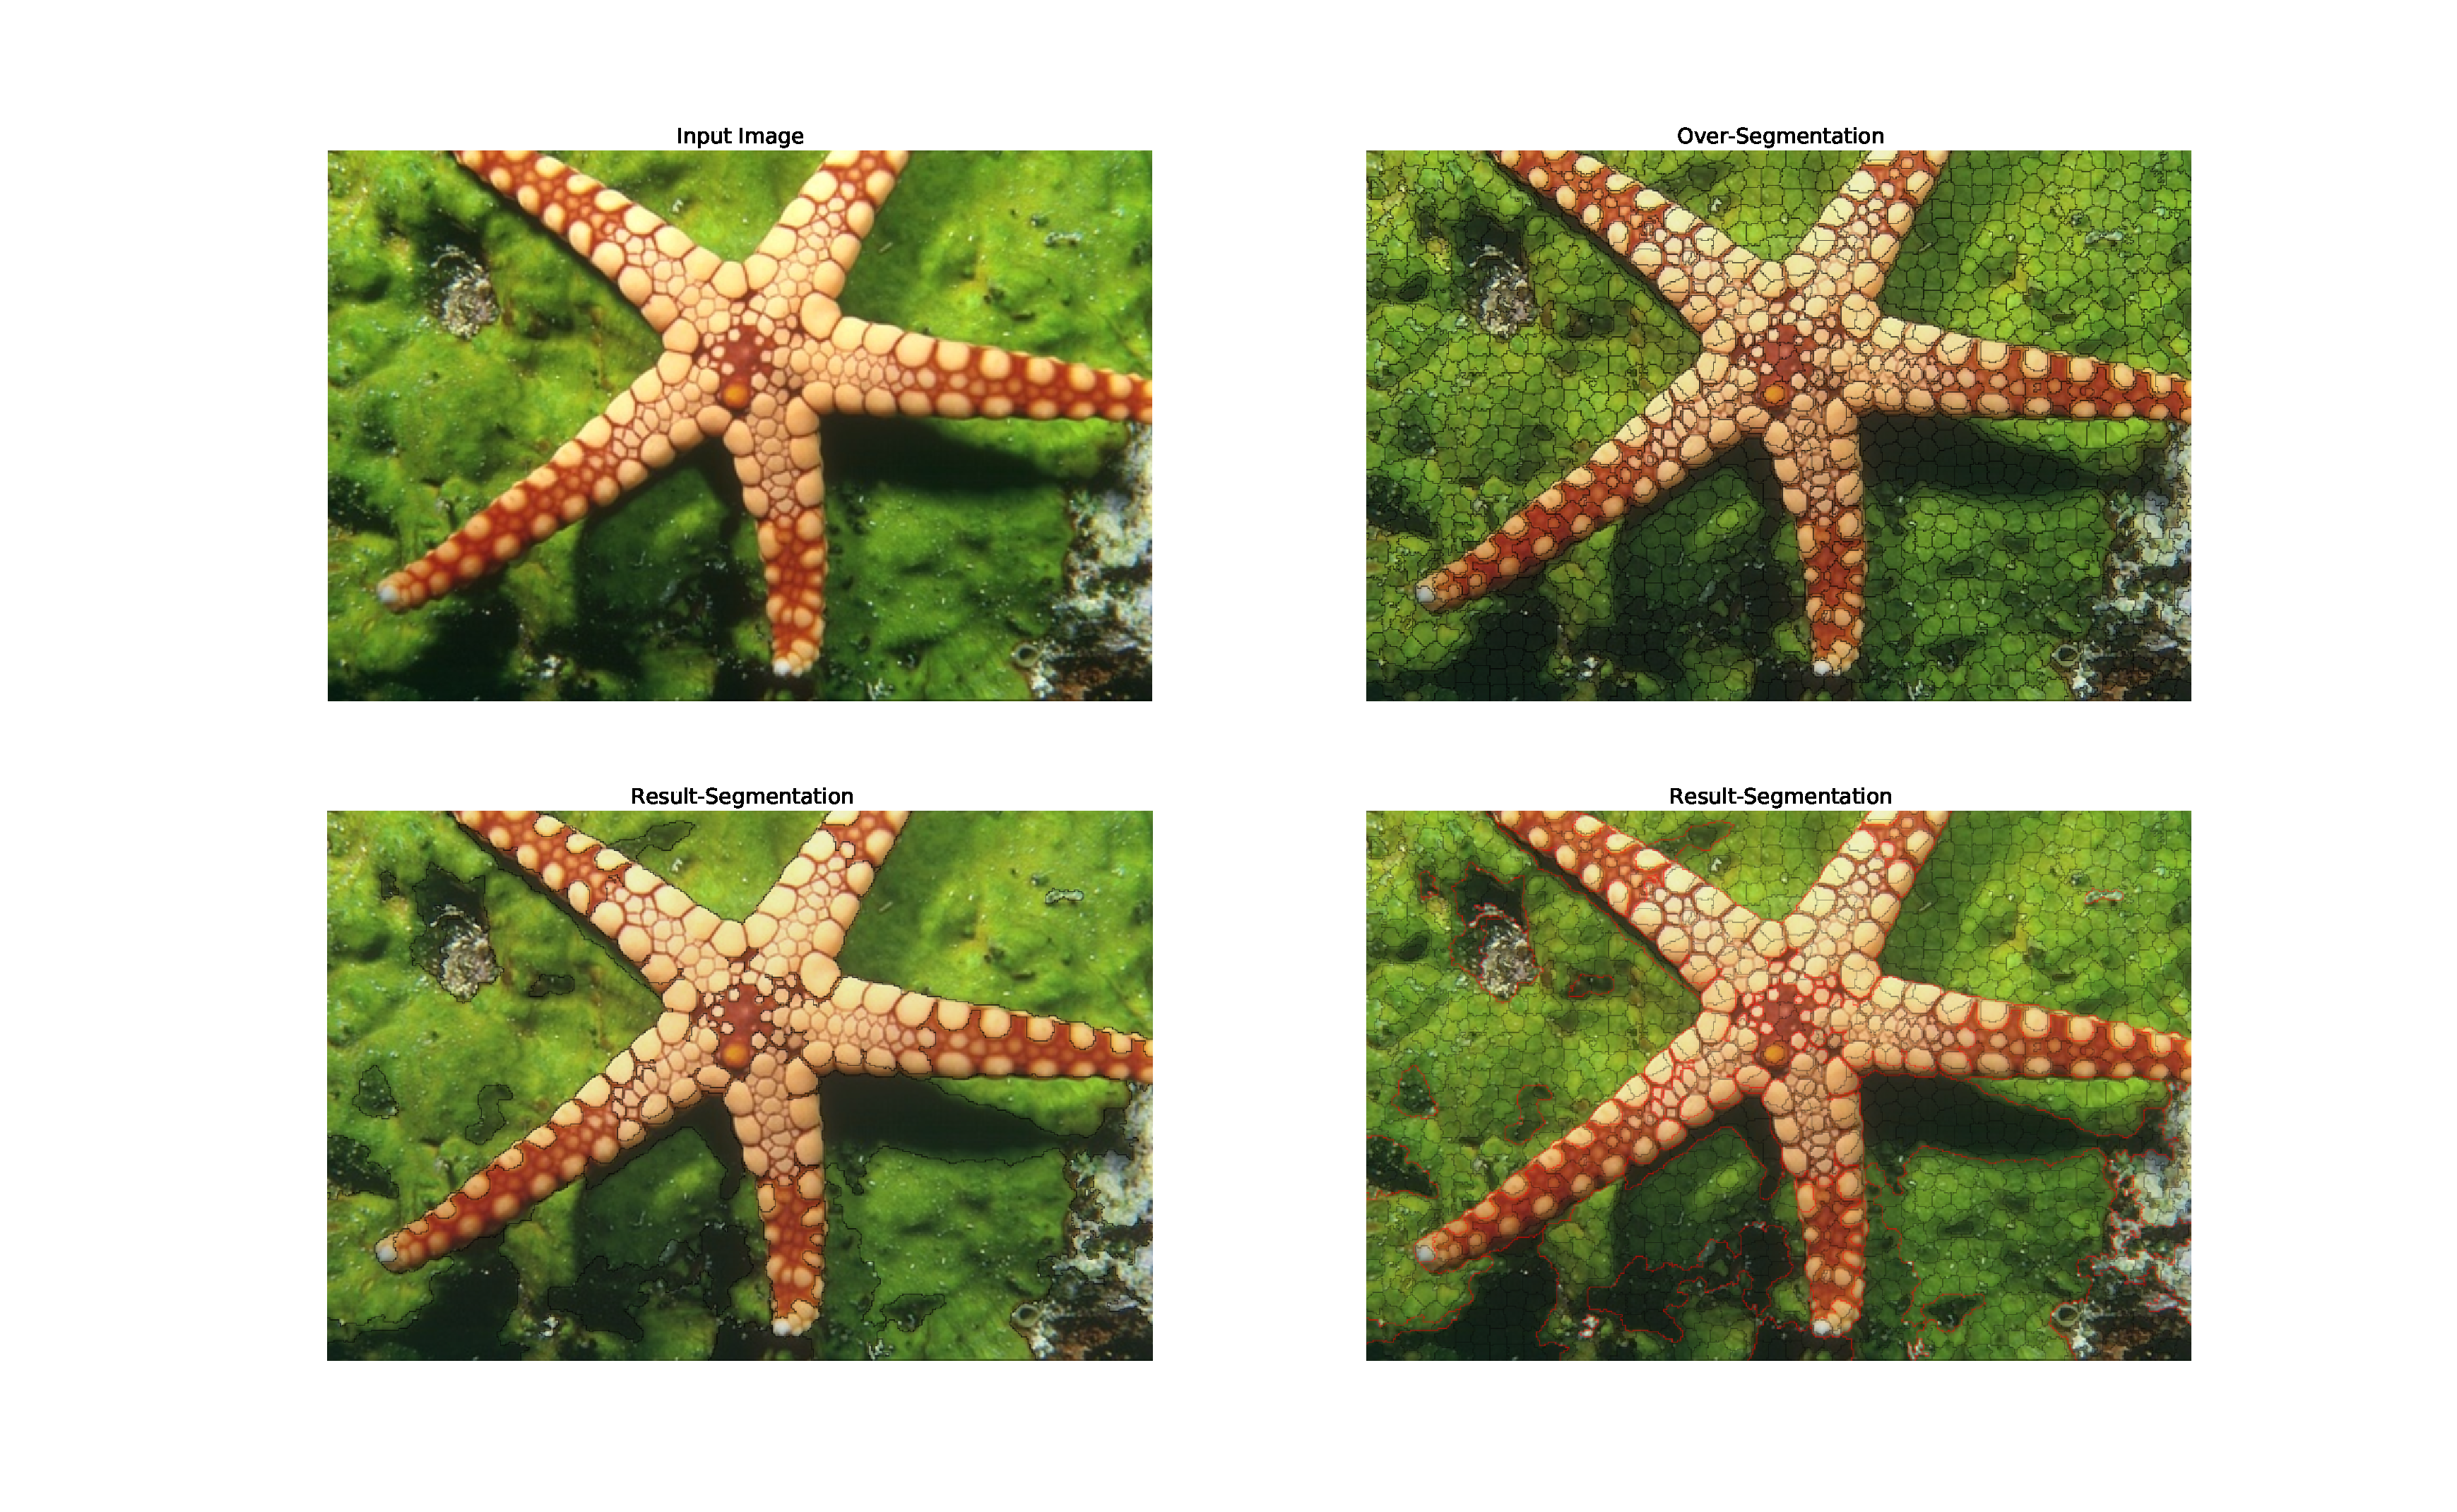
\includegraphics[width=\textwidth]{fig/res_hcluster.pdf}
\end{figure}


%\paragraph{Graph Smoothing}
%\lstinputlisting[language=Python]
%{/home/tbeier/src/vigra/vigranumpy/examples/graph_smoothing.py}

\paragraph{Felzenszwalb}
In this example we show how to use the method 
proposed by \citet{felzenszwalb_2004_ijcv}.
\lstinputlisting[language=Python]
{/home/tbeier/src/vigra/vigranumpy/examples/graph_felzenszwalb.py}

\paragraph{Watersheds}
In this example we show how to use edge and node weighted
watersheds.
To make both comparable, we use the same seeds for both.
The evaluation map is based on the gradient magnitude.

\lstinputlisting[language=Python]
{/home/tbeier/src/vigra/vigranumpy/examples/graph_watersheds.py}